\documentclass[a4paper,10pt]{article}
\usepackage[utf8]{inputenc}
\usepackage[T1]{fontenc}
\usepackage[english]{babel}
\usepackage[a4paper,top=2.5cm, bottom=2.5cm, left=2.5cm, right=2.5cm]{geometry}
\usepackage{graphicx}

\title{Software Architectures\\ Assignment 1 : Design Patterns}
\author{Arnaud Rosette, Simon Picard}

\begin{document}
\maketitle
\section{Exercise 1 : Find Instances of Design Patterns}
\subsection{Singleton}%org.gjt.sp.jedit.syntax.ModeProvider
The org.gjt.sp.jedit.buffer.KillRing class is an instance of the singleton pattern.

\subsubsection{Purpose}
Creational pattern.
\subsubsection{Participants}
The KillRing class is the singleton class.
\subsubsection{Class diagram}
\begin{center}
\begin{figure}[h]
  \centerline{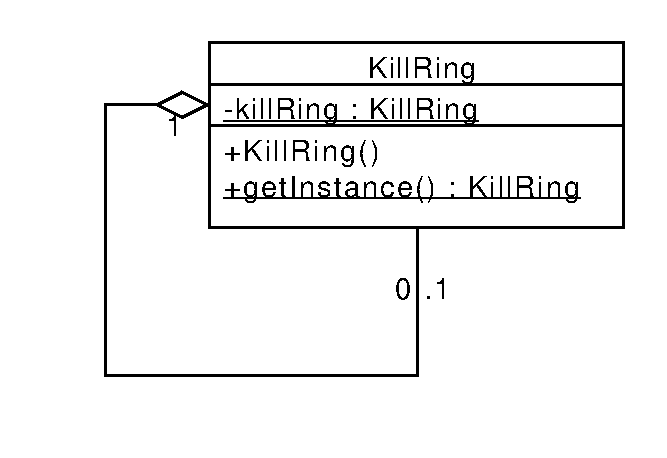
\includegraphics[width=0.5\textwidth]{singleton-killring-class-diagram.pdf}}
  \caption{KillRing class diagram}
\end{figure}
\end{center}
\subsubsection{Concrete situation description}
In this situation, the singleton pattern is used to keep track of deleted text in a single place in the application.\\
The constructor is here public. However, the common usage of the singleton pattern uses a private constructor in order to only have one instance of this class living in the system. The constructor is here made public because the plugins may want to create their own KillRing. 


\subsection{Abstract Factory}%org.gjt.sp.jedit.syntax.ModeProvider, org.gjt.sp.jedit.io.VFSManager, org.gjt.sp.jedit.gui.statusbar.StatusWidgetFactory (abstract factory) avec BufferSetWidgetFactory (concrete factory) avec Widget (abstract product) avec org.gjt.sp.jedit.gui.StatusBar (client)
The org.gjt.sp.jedit.gui.statusbar.StatusWidgetFactory is an example of the abstract factory pattern.

\subsubsection{Purpose}
Creational pattern.
\subsubsection{Participants}
The participants are the classes : org.gjt.sp.jedit.gui.statusbar.StatusWidgetFactory, org.gjt.sp.jedit.gui.statusbar.BufferSetWidgetFactory, org.gjt.sp.jedit.gui.statusbar.BufferSetWidget, org.gjt.sp.jedit.gui.statusbar.Widget and org.gjt.sp.jedit.gui.StatusBar.

\begin{itemize}
 \item \textbf{StatusWidgetFactory} : Abstract Factory
 \item \textbf{BufferSetWidgetFactory} : Concrete Factory
 \item \textbf{BufferSetWidget} : Concrete Product
 \item \textbf{Widget} : Abstract Product
 \item \textbf{StatusBar} : Client
\end{itemize}

\subsubsection{Class diagram}
\begin{center}
\begin{figure}[h]
  \centerline{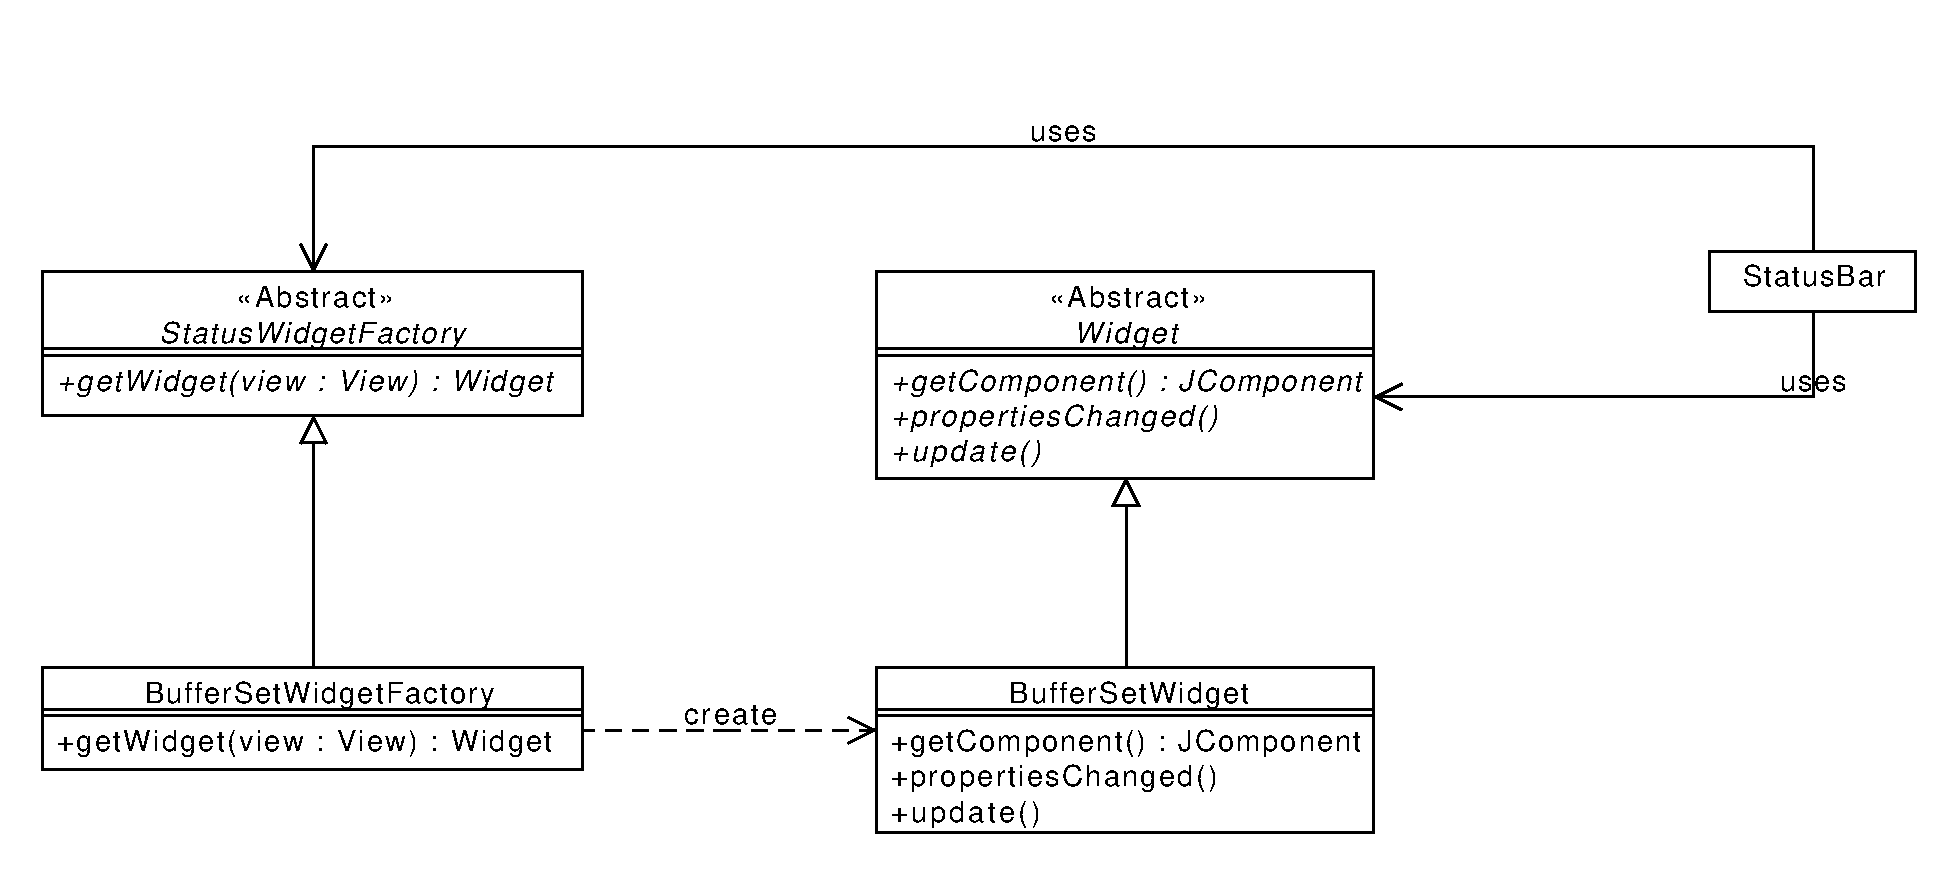
\includegraphics[width=0.7\textwidth]{abstractfactory-statuswidgetfactory-class-diagram.pdf}}
  \caption{StatusWidgetFactory class diagram}
\end{figure}
\end{center}
\subsubsection{Concrete situation description}
In this situation, the abstract factory pattern is used to let a StatusBar object creating different kind of Widget without specifying their concrete class. 

\subsection{Observer}

\subsubsection{Purpose}

\subsubsection{Participants}

\subsubsection{Class diagram}

\subsubsection{Concrete situation description}


\subsection{Adapter}
The org.gjt.sp.jedit.buffer.BufferAdapter is an example of the adapter pattern.

\subsubsection{Purpose}
Structural pattern.
\subsubsection{Participants}
The participants are the classes : org.gjt.sp.jedit.buffer.BufferAdapter, org.gjt.sp.jedit.buffer.BufferListener, a client and a target.
\begin{itemize}
 \item \textbf{BufferAdapter} : Adapter
 \item \textbf{BufferListener} : Adaptee
\end{itemize}

\subsubsection{Class diagram}

\subsubsection{Concrete situation description}


\subsection{Visitor}

\subsubsection{Purpose}

\subsubsection{Participants}

\subsubsection{Class diagram}

\subsubsection{Concrete situation description}


\end{document}
